% =====================================================================
% Springer Nature (sn-jnl) template conversion
% Paper: Kelvin Mode Suppression in Atomic Orbitals: A Vortex-Filament Gap
% Author: Omar Iskandarani
% Date (source): 2025-12-14
% Affiliation: Independent Researcher, Groningen, The Netherlands
% License: © 2025 Omar Iskandarani. All rights reserved.
% DOI: 10.5281/zenodo.18018084
% =====================================================================

% =========================
% 1) Document class choice
% =========================
% \documentclass[referee,pdflatex,sn-mathphys-num]{sn-jnl} % double-spacing option for review
\documentclass[pdflatex,sn-mathphys-num]{sn-jnl}

% =========================
% 2) Core packages (lean)
% =========================
\usepackage[T1]{fontenc}
\usepackage[utf8]{inputenc}
\usepackage{lmodern}
\usepackage{microtype}
\usepackage{graphicx}
\usepackage{booktabs}
\usepackage{amsmath,amssymb,amsfonts}
\usepackage{bm}
\usepackage{siunitx}
% \usepackage{physics}

% TikZ/PGFPlots (used by your figures)
\usepackage{tikz}
\usepackage{pgfplots}
\usepackage{pgfplotstable}
\usepackage{caption}
\pgfplotsset{compat=newest}

% ====================================
% 3) Paper metadata macros (edit here)
% ====================================
\newcommand{\papertitle}{Spectroscopic Constraints on Kelvin-Like Internal Modes in Effective Filament Models of Atomic Bound States}
\newcommand{\papershorttitle}{Kelvin-Like Internal Modes in Atomic Bound States}
\newcommand{\paperdoi}{10.5281/zenodo.18018084}
\newcommand{\paperorcid}{0009-0006-1686-3961}
\newcommand{\paperemail}{info@omariskandarani.com}
\newcommand{\papercity}{Groningen}
\newcommand{\papercountry}{The Netherlands}
\newcommand{\paperkeywords}{Kelvin modes, effective filament models, atomic spectroscopy, excitation gap, low-energy reduction}

\raggedbottom

\begin{document}

% =========================
% 5) Title + author block
% =========================
    \title[\papershorttitle]{\papertitle}

    \author*[1]{\fnm{Omar} \sur{Iskandarani}}\email{\paperemail}
    \affil*[1]{\orgname{Independent Researcher}, \orgaddress{\city{\papercity}, \country{\papercountry}}}

% =========================
% 6) Abstract + keywords
% =========================
    \abstract{%
        We consider effective atomic bound-state models supplemented by an internal helical excitation sector with Kelvin-like dispersion. The central question is whether such an internal sector can remain compatible with precision atomic spectroscopy. We obtain a conditional decoupling bound: if the internal spectrum is separated from the orbital sector by an excitation gap $\Delta_K$, then the induced correction is Boltzmann suppressed, $\delta E_n \propto \exp[-\Delta_K/(k_B T_{\mathrm{eff}})]$, and the low-energy orbital description remains spectroscopically stable. By contrast, ungapped constructions do not enjoy generic exponential protection and therefore require additional suppression mechanisms to remain compatible with spectroscopy. The resulting constraint is conditional on the effective occupation scale $T_{\mathrm{eff}}$, the active mode count $N_K$, and the coupling efficiency $\lambda_n$. A separate dispersion-based estimate places the onset of the lowest internal mode in a geometry-dependent window spanning roughly $10^2\,\mathrm{eV}$ to $10^3\,\mathrm{eV}$ for the fiducial parameter sweep presented in Appendix~A. Taken together, the spectroscopy bound and the onset estimate define a consistency window rather than a unique prediction.%
    }

    \keywords{\paperkeywords}

    \maketitle

% Global dimensionless temperature ratio
    \newcommand{\epsilonK}{\varepsilon_K} % Dimensionless temperature ratio

% ============================================================
    \section{Introduction}\label{sec:intro}
        Hydrodynamic and vortex-based models of matter trace back to Kelvin and Helmholtz \cite{Helmholtz1858,Kelvin1867}. Modern superfluid dynamics and quantum turbulence have renewed interest in vortex filaments as fundamental excitations \cite{Onsager1949,Feynman1955,Barenghi2014}.

        In that broader context, it is natural to ask whether an atomic bound state might admit an \emph{effective} description in which the usual orbital degree of freedom is accompanied by an internal filament-like excitation sector.

        This paper does not attempt to establish such a microscopic picture as fundamental. Its purpose is narrower: to derive a consistency condition. If an internal Kelvin-like sector exists and couples to bound electronic states, then atomic spectroscopy immediately constrains its low-energy behavior. The question is therefore not whether one prefers a filament interpretation, but whether any such internal sector can remain invisible at atomic energies.

        The main result is narrower than a no-go theorem. An ungapped Kelvin-like spectrum does not enjoy any generic exponential protection, so compatibility with spectroscopy requires additional suppression from the density of states, the effective occupation scale, or the coupling to observable line shifts. A gapped spectrum avoids this problem: below the gap, the internal sector is effectively frozen and only a Boltzmann-suppressed correction survives. The paper should therefore be read as establishing a conditional consistency bound for internal-mode completions of atomic bound states rather than as ruling out all ungapped constructions in full generality.

% ============================================================
    \section{Kelvin Waves on Vortex Filaments}\label{sec:kelvin}
        For a thin filament with circulation $\Gamma$ and core radius $\xi$, small-amplitude Kelvin waves satisfy \cite{LordKelvin1880,Barenghi2014}
        \begin{equation}
            \omega(k) \simeq \frac{\Gamma}{4\pi} k^2
            \left[
                \ln\!\left(\frac{1}{|k|\xi}\right) + C_0
            \right],
            \label{eq:kelvin_dispersion}
        \end{equation}
        with $C_0=\mathcal{O}(1)$. For a closed filament of length $L$,
        \begin{equation}
            k_m = \frac{2\pi m}{L}, \quad m=1,2,\dots,\qquad
            \omega_m \propto \frac{\Gamma m^2}{L^2}.
        \end{equation}
        Here the logarithmic factor from Eq.~\eqref{eq:kelvin_dispersion} is suppressed only for compactness; in the parameter regime relevant below, $\ln\!\bigl(1/(|k_m|\xi)\bigr)+C_0$ is retained in all explicit numerical estimates and contributes at order unity to order ten. For hydrogenic orbitals $r_n=a_0 n^2$, implying $L_n\sim 2\pi a_0 n^2$, Kelvin frequencies soften rapidly with principal quantum number $n$.

% ============================================================
    \section{Thermodynamic Constraint from Atomic Spectroscopy}\label{sec:constraint}
        Suppose an atomic bound state carries, in addition to its orbital energy $E_n^{(0)}$, an internal contribution from Kelvin-like modes,
        \begin{equation}
            E_n^{\mathrm{eff}}(T_{\mathrm{eff}})
            =
            E_n^{(0)} + \delta E_n(T_{\mathrm{eff}}),
        \end{equation}
        where $T_{\mathrm{eff}}$ is not necessarily a literal thermodynamic temperature, but an effective population scale for the internal sector.

        The key physical assumption is that internal excitation energy can feed into an observed level shift with some efficiency $\lambda_n$. A convenient generic parametrization is
        \begin{equation}
            |\delta E_n(T_{\mathrm{eff}})|
            \le
            \lambda_n \sum_m E_{m,n}\, \nu_{m,n}(T_{\mathrm{eff}}),
            \qquad 0\le \lambda_n \le 1,
            \label{eq:generic_coupling_bound}
        \end{equation}
        where $E_{m,n}$ are internal mode energies and $\nu_{m,n}$ are occupation factors. The present paper does not derive $\lambda_n$ microscopically; rather, it keeps that coupling explicit so that the resulting constraint can be read conditionally.

        In an ungapped sector, low-energy modes can in principle be populated down to arbitrarily small excitation energy, and no generic exponential suppression follows. Compatibility with spectroscopy would then require additional structure, such as a strongly depleted low-energy density of states, a very small effective occupation scale, or a very weak coupling $\lambda_n$ to observable line shifts. By contrast, once the internal spectrum is gapped, the induced correction acquires Boltzmann suppression, which is the only ingredient needed for the consistency bound derived below.

% ============================================================
    \section{Gapped Kelvin Spectrum}\label{sec:gap}
        The minimal decoupling mechanism is an excitation gap $\Delta_K$ in the internal spectrum: the first excitation costs $\Delta_K$, and higher modes obey $E_{m,n}\ge\Delta_K$. Near a stable closed-filament configuration, the small-amplitude internal excitations may be parametrized as independent normal modes; the minimal harmonic representation is
        \begin{equation}
            H_K^{(n)} = \sum_m \left[
                                   (\Delta_K+\delta E_{m,n})\, b_{mn}^\dagger b_{mn}
                                   + \frac{1}{2}(\Delta_K+\delta E_{m,n})
            \right].
        \end{equation}
        This Hamiltonian is used only as an effective normal-mode parametrization of a gapped internal sector, not as a microscopic derivation from first principles. The microscopic origin of $\Delta_K$ is left open here; in an effective filament picture it may arise from topology, curvature, torsion, core structure, or geometric constraints on admissible excitations \cite{Ricca1996}.

        A dimensional estimate supports the required magnitude of $\Delta_K$. For a filament with circulation $\Gamma$ and core radius $\xi$, the tension $T_f \sim \rho \, \Gamma^2/(4\pi \xi^2)$ sets a characteristic bending energy for the first Kelvin mode. Taking the mode wavelength to be of order the loop length $L$, one obtains $\Delta_K \sim \Gamma^2/(4\pi \xi L)$ up to logarithmic corrections. With $\Gamma = h/m_e$, $\xi \sim 10^{-15}\,\mathrm{m}$, and $L \sim 10^{-10}\,\mathrm{m}$, this gives $\Delta_K = \mathcal{O}(10^2\text{--}10^3\,\mathrm{eV})$, consistent with the phenomenological scale used below.

% ============================================================
    \section{Low-Temperature Thermodynamics}\label{sec:lowT}
        The dimensionless temperature ratio
        \[
            \epsilonK = \frac{k_B T}{\Delta_K} \ll 1
        \]
        characterizes the low-temperature (Kelvin-frozen) regime.
        For a single gapped bosonic mode \cite{Pathria2011},
        \begin{equation}
            Z = \frac{1}{1 - e^{-\beta\Delta_K}}, \qquad
            U = \frac{\Delta_K}{e^{\beta\Delta_K} - 1}, \qquad
            \beta = (k_B T)^{-1}.
        \end{equation}
        In the limit $\epsilonK \ll 1$,
        \begin{equation}
            U \simeq \Delta_K e^{-1/\epsilonK},
        \end{equation}
        so entropy and heat capacity are exponentially suppressed.

        \begin{figure}[htbp]
            \centering
            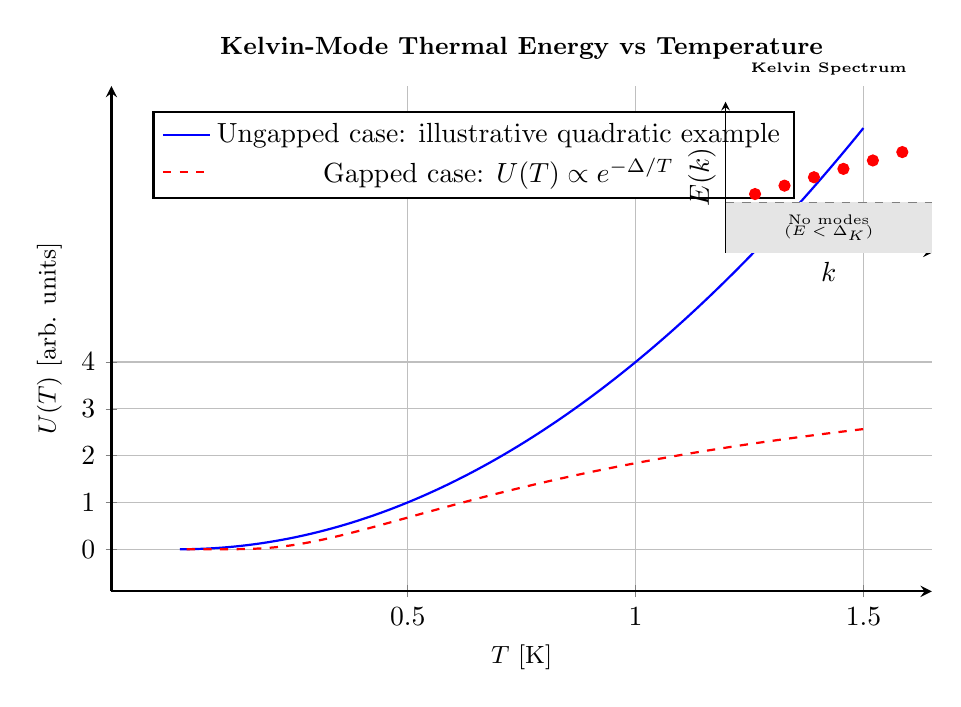
\begin{tikzpicture}
% MAIN PLOT: Thermal Energy vs Temperature
                \begin{axis}[
                width=12cm,
                height=8cm,
                xlabel={$T$ [K]},
                ylabel={$U(T)$ [arb. units]},
                legend style={at={(0.05,0.95)}, anchor=north west},
                domain=0:1.5,
                samples=100,
                axis lines=left,
                enlargelimits=true,
                grid=both,
                xtick={0.5,1.0,1.5},
                ytick={0,1,2,3,4},
                xlabel style={font=\small},
                ylabel style={font=\small},
                title={Kelvin-Mode Thermal Energy vs Temperature},
                title style={font=\bfseries\small},
                thick
                ]
% No Gap: U ~ T^2
                \addplot[blue,thick] {4*x^2};
                \addlegendentry{Ungapped case: illustrative quadratic example}
% With Gap: U ~ exp(-Δ/T)
                \addplot[red,thick,dashed] {5*exp(-1/x)};
                \addlegendentry{Gapped case: $U(T) \propto e^{-\Delta/T}$}
                \end{axis}

% INSET: Energy spectrum with gap
                \begin{scope}[shift={(7.8,4.3)}]
                    \begin{axis}[
                    width=4.2cm,
                    height=3.5cm,
                    title={Kelvin Spectrum},
                    title style={font=\bfseries\tiny},
                    xlabel={$k$},
                    ylabel={$E(k)$},
                    axis lines=left,
                    ticks=none,
                    xmin=0, xmax=3.5,
                    ymin=0, ymax=4.5,
                    xtick=\empty,
                    ytick=\empty,
                    clip=false
                    ]
                    \fill[gray!20] (axis cs:0,0) rectangle (axis cs:3.5,1.5);
                    \draw[dashed, gray] (axis cs:0,1.5) -- (axis cs:3.5,1.5);
                    \foreach \x in {0.5,1.0,1.5,2.0,2.5,3.0} {
                        \addplot[only marks, mark=*, red] coordinates {(\x, {1.5 + 0.5*\x})};
                    }
                    \node[align=center,font=\tiny] at (axis cs:1.75,0.75) {No modes\\[-0.3em]($E<\Delta_K$)};
                    \end{axis}
                \end{scope}
            \end{tikzpicture}
            \caption{Comparison of Kelvin-mode thermal energy with and without an excitation gap $\Delta_K$. The ungapped curve is an illustrative quadratic example only and does not assert a universal $T^2$ law. Inset: discrete spectrum with a forbidden band $E<\Delta_K$.}
            \label{fig:kelvin-gap}
        \end{figure}

        \begin{figure}[htbp]
            \centering
            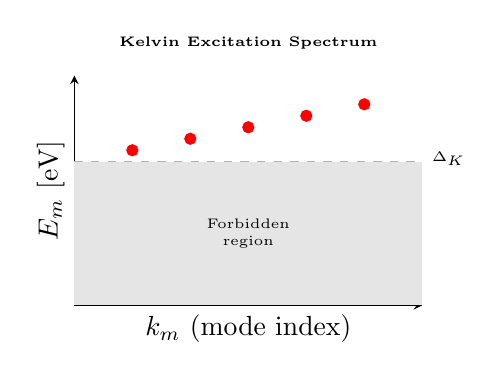
\begin{tikzpicture}
                \begin{axis}[
                width=6cm,
                height=4.5cm,
                title={Kelvin Excitation Spectrum},
                title style={font=\bfseries\tiny},
                xlabel={$k_m$ (mode index)},
                ylabel={$E_m$ [eV]},
                axis lines=left,
                ticks=none,
                xmin=0, xmax=6,
                ymin=0, ymax=800,
                clip=false
                ]
                \pgfmathsetmacro{\DeltaK}{500} % eV gap
                \fill[gray!20] (axis cs:0,0) rectangle (axis cs:6,\DeltaK);
                \draw[dashed, gray!60] (axis cs:0,\DeltaK) -- (axis cs:6,\DeltaK);
                \node[align=center,font=\tiny] at (axis cs:3,250) {Forbidden\\ region};
                \foreach \x in {1,2,3,4,5} {
                    \addplot[only marks, mark=*, red, mark size=2pt] coordinates {(\x, {\DeltaK + 40*\x})};
                }
                \node[anchor=west,font=\tiny] at (axis cs:6,\DeltaK+10) {$\Delta_K$};
                \end{axis}
            \end{tikzpicture}
            \caption{Illustrative Kelvin excitation spectrum with a gap $\Delta_K=\SI{500}{\electronvolt}$. Shaded band: $E<\Delta_K$.}
            \label{fig:kelvin-thermal-suppression}
        \end{figure}

        For finitely many Kelvin modes,
        \begin{equation}
            U_K^{(n)}(T) \lesssim N_K \Delta_K \exp\!\left(-\frac{\Delta_K}{k_B T}\right),
        \end{equation}
        replacing the dangerous polynomial scaling of the ungapped case.

% ============================================================
    \section{Required Gap Scale}\label{sec:required_gap}
        Let $\delta E_{\mathrm{spec}}$ denote the maximum spectroscopy-compatible correction to a low-lying level. For a finite or effectively truncated active mode set of size $N_K$, Eq.~\eqref{eq:generic_coupling_bound} together with Boltzmann suppression gives the sufficient decoupling condition
        \begin{equation}
            \lambda_n N_K \Delta_K
            \exp\!\left(-\frac{\Delta_K}{k_B T_{\mathrm{eff}}}\right)
            \lesssim
            \delta E_{\mathrm{spec}}.
            \label{eq:general_bound}
        \end{equation}
        Equivalently,
        \begin{equation}
            \frac{\Delta_K}{k_B T_{\mathrm{eff}}}
            \gtrsim
            \ln\!\left(\frac{\lambda_n N_K \Delta_K}{\delta E_{\mathrm{spec}}}\right).
            \label{eq:log_bound}
        \end{equation}
        The dependence on $\lambda_n$, $N_K$, and $\delta E_{\mathrm{spec}}$ is only logarithmic. The numerical non-triviality of Eq.~\eqref{eq:log_bound} therefore depends primarily on the assumed effective occupation scale $T_{\mathrm{eff}}$ and on the coupling efficiency $\lambda_n$: for room-temperature populations or extremely weak coupling, the bound may require only an eV-scale gap, whereas substantially larger $T_{\mathrm{eff}}$ and order-unity coupling push the required gap above ordinary atomic binding energies. The present paper does not independently derive a specific range for $T_{\mathrm{eff}}$, nor does it provide a microscopic estimate of $\lambda_n$; accordingly, Eq.~\eqref{eq:log_bound} should be read strictly as a conditional constraint on parameter space rather than as an absolute numerical prediction. Appendix~\ref{app:first_kelvin} then supplies an independent fiducial onset estimate for the lowest internal mode. Taken together, the spectroscopic bound and the dispersion estimate define a consistency window rather than a sharp prediction.

% ============================================================
    \section{Discussion and Outlook}\label{sec:outlook}
        The result of this paper is a conditional consistency bound. Any effective atomic bound-state model endowed with an internal Kelvin-like filament sector faces a sharp spectroscopic requirement: once the parameters $(\lambda_n,N_K,T_{\mathrm{eff}},\Delta_K)$ and the spectroscopic tolerance $\delta E_{\mathrm{spec}}$ are specified, Eq.~\eqref{eq:log_bound} determines whether the internal sector is safely decoupled from observed low-energy lines. A nonzero gap provides exponential protection. An ungapped sector can still be compatible with spectroscopy, but only if some additional mechanism suppresses either the low-energy density of states, the effective occupation, or the coupling to observed level shifts.

        The non-triviality of the bound depends explicitly on the same unresolved microscopic inputs. In particular, the constraint is physically informative only in regimes where the coupling efficiency $\lambda_n$ is not itself extremely suppressed. If $\lambda_n \ll 1$---for example, exponentially small in the relevant control parameters---or if no physical process populated the internal sector above a negligible effective scale, the constraint would become correspondingly weak even for modest $\Delta_K$. Determining whether $\lambda_n$ is of order unity, perturbatively small, or parametrically tiny is therefore a microscopic question for any specific filament model and lies beyond the scope of the present phenomenological note, but such a mechanism would set how restrictive Eq.~\eqref{eq:log_bound} becomes in practice.

        This framing yields a narrow and testable claim. The relevant experimental question is not whether atomic structure is ``really'' filamentary, but whether any additional internal sector activates above a threshold lying in the appendix's fiducial window,
        \begin{equation}
            10^2\,\mathrm{eV} \lesssim \Delta_K \lesssim 10^3\,\mathrm{eV},
        \end{equation}
        for the illustrative parameter choices considered there. Potential signatures would then appear not in ordinary spectroscopy, where the sector is frozen, but in threshold-like inelastic channels, anomalous broadening, or additional loss mechanisms once the excitation scale is crossed.

        The paper therefore motivates a focused search strategy: high-field or high-energy probes of bound electrons, rather than reinterpretation of standard low-energy spectroscopy. At low energy the internal sector must be silent; at sufficiently high excitation, it may become observable.

% ============================================================
        \appendix
    \section*{Appendix A: Estimate of First Kelvin Mode Energy}\label{app:first_kelvin}
        For the first mode ($m=1$) in the ground state ($n=1$), take
        \begin{equation}
            L = 2\pi a_0 \approx \SI{3.3249e-10}{m},
            \qquad
            \Gamma = \frac{h}{m_e} \approx \SI{7.2739e-4}{m^2/s},
        \end{equation}
        so that
        \begin{equation}
            k_1 = \frac{2\pi}{L} \approx \SI{1.8897e10}{m^{-1}}.
        \end{equation}
        For general regularization length $\xi$ and core constant $C_0$,
        \begin{equation}
            \omega_1(\xi,C_0,L)
            \simeq
            \frac{\Gamma}{4\pi} k_1^2
            \left[
                \ln\!\left(\frac{1}{k_1 \xi}\right) + C_0
            \right],
        \end{equation}
        and
        \begin{equation}
            E_1(\xi,C_0,L)=\hbar \omega_1(\xi,C_0,L).
        \end{equation}

        With the fiducial choice $\xi=\SI{1e-15}{m}$ and $C_0=1$, Eq.~\eqref{eq:kelvin_dispersion} yields
        \begin{equation}
            \omega_1 \approx \SI{2.45e17}{rad/s},
            \qquad
            E_1 \approx \SI{1.62e2}{eV}.
        \end{equation}

        Because the estimate depends on both the regularization scale $\xi$ and the effective loop length $L$, it is useful to display that sensitivity explicitly. For fixed $L=2\pi a_0$ and $C_0=1$:
        \begin{table}[htbp]
            \centering
            \caption{Sensitivity of the first-mode onset estimate to the regularization scale $\xi$ at fixed $L=2\pi a_0$ and $C_0=1$.}
            \begin{tabular}{ccc}
                \toprule
                $\xi$ [m] & $\ln(1/k_1\xi)+1$ & $E_1$ [eV] \\
                \midrule
                $10^{-15}$ & 11.876 & 162 \\
                $10^{-14}$ & 9.573  & 131 \\
                $10^{-13}$ & 7.271  & 99  \\
                \bottomrule
            \end{tabular}
            \label{tab:xi-sensitivity}
        \end{table}

        Likewise, at fixed $\xi=\SI{1e-15}{m}$ and $C_0=1$, shortening the effective loop length raises the onset scale:
        \begin{table}[htbp]
            \centering
            \caption{Sensitivity of the first-mode onset estimate to the effective loop length $L$ at fixed $\xi=\SI{1e-15}{m}$ and $C_0=1$.}
            \begin{tabular}{ccc}
                \toprule
                $L$ & $k_1$ [m$^{-1}$] & $E_1$ [eV] \\
                \midrule
                $2\pi a_0$      & $1.89\times 10^{10}$ & 162  \\
                $\pi a_0$       & $3.78\times 10^{10}$ & 587  \\
                $\tfrac{2\pi a_0}{3}$ & $5.67\times 10^{10}$ & 1320 \\
                \bottomrule
            \end{tabular}
            \label{tab:L-sensitivity}
        \end{table}

        For the illustrative parameter sweep reported above, the onset window may therefore be summarized as
        \begin{equation}
            \SI{1e2}{\electronvolt} \lesssim E_1 \lesssim \SI{1.3}{\kilo\electronvolt}.
        \end{equation}
        This window is not a unique prediction. It is a sensitivity range obtained from the Kelvin dispersion relation once the regularization scale $\xi$, the effective loop length $L$, and the order-unity core constant $C_0$ are specified. The dispersion estimate therefore supplies a fiducial onset scale together with a geometry-dependent consistency window, which is the sense in which it supports the main text.

% ============================================================
% Back matter (Springer Nature)
% ============================================================
        \backmatter
        \bmhead{Declarations}

        \subsection*{Funding}
            Not applicable.

        \subsection*{Competing interests}
            The author declares no competing interests.

        \subsection*{Ethics approval}
            Not applicable.

        \subsection*{Consent to participate}
            Not applicable.

        \subsection*{Consent for publication}
            Not applicable.

        \subsection*{Data availability}
            Not applicable.

        \subsection*{Materials availability}
            Not applicable.

        \subsection*{Code availability}
            Not applicable.

        \subsection*{Author contributions}
            O.I. conceived the study, developed the analysis, performed the derivations, and wrote the manuscript.

% ============================================================
% References
% ============================================================
            \begin{thebibliography}{99}

                \bibitem{Helmholtz1858}
                H.~Helmholtz,
                ``On Integrals of the Hydrodynamical Equations Which Express Vortex Motion,''
                \emph{J. Reine Angew. Math.} \textbf{55}, 25--55 (1858).

                \bibitem{Kelvin1867}
                W.~Thomson (Lord Kelvin),
                ``On Vortex Atoms,''
                \emph{Proc. R. Soc. Edinburgh} \textbf{6}, 94--105 (1867).

                \bibitem{Onsager1949}
                L.~Onsager,
                ``Statistical Hydrodynamics,''
                \emph{Nuovo Cimento Suppl.} \textbf{6}, 279--287 (1949).

                \bibitem{Feynman1955}
                R.~P.~Feynman,
                ``Application of Quantum Mechanics to Liquid Helium,''
                in \emph{Progress in Low Temperature Physics}, Vol.~1,
                North-Holland (1955).

                \bibitem{LordKelvin1880}
                W.~Thomson (Lord Kelvin),
                ``Vibrations of a Columnar Vortex,''
                \emph{Philosophical Magazine} \textbf{10}, 155--168 (1880).

                \bibitem{Barenghi2014}
                C.~F.~Barenghi, L.~Skrbek, and K.~R.~Sreenivasan,
                ``Introduction to Quantum Turbulence,''
                \emph{Proc. Natl. Acad. Sci. USA} \textbf{111}, 4647--4652 (2014).

                \bibitem{Ricca1996}
                R.~L.~Ricca,
                ``The Contributions of Da Rios and Levi-Civita to Asymptotic Potential Theory and Vortex Filament Dynamics,''
                \emph{Fluid Dynamics Research} \textbf{18}, 245--268 (1996).

                \bibitem{Pathria2011}
                R.~K.~Pathria and P.~D.~Beale,
                \emph{Statistical Mechanics}, 3rd ed.,
                Elsevier (2011).

            \end{thebibliography}

\end{document}